\documentclass[12pt]{article}
\usepackage[utf8]{inputenc}
\usepackage[margin=1in]{geometry}

\usepackage{biblatex}
\usepackage{indentfirst}
\usepackage{amsmath}
\usepackage{graphicx}
\usepackage{caption}
\usepackage{subcaption}
\usepackage{hyperref}

\graphicspath{ {images/} }

\renewcommand{\baselinestretch}{1.2}

\title{Discovering Panoramas in Web Videos \\ lhuang58.github.io}

\author{Lingfeng Huang, Fang Wang}
\date{11/2016}

\begin{document}
\maketitle

\section*{Abstract}
Panoramas have been widely used in may applications in multimedia, but the main constraint for panoramas is that they must be
taken by people who physically present at the place. In this project, we will implement our version of Discovering Panoramas in Web Videos by Liu et al. 
to solve the problem by selecting optimal segments within a given web videos, then perform synthesizing to obtain panoramas. This 
whole procedure is basically a optimization problem where we optimize the three criteria which are wide field of view, mosaicability, and high image 
quality.
\section{Introduction}
The emerge of the idea "Panorama" has to be dated back to early 20 A.D. and was a means of generating an 'panoptic' view of a vista \cite{wikipedia}. Nowadays, 
with the help of advancement of technology, people are able to create desired panorama by simply rotating their cell phones and clicking the shot button. The process
of synthesizing panorama is relatively straight forward. First step is to take successive photos from the same optical center and next step is finding the alignment between
each image and warping accordingly, and final step is interpolating the warped image and applied certain blending to remove the visible seams. However, the problem with creating
panoramas using above approach is that people are required to physically appear at the place where they take the images, which means that if people want to take a panorama
of Time Square in New York, they have to fly over New York to do so. \par
Compared to sequence of images, although some segments within videos have relatively low image quality and also moving object, they are still shot from the same optical center and cover a wide field-of-view. Lui et al. suggests an approach that synthesizing panoramas by identifying proper segments within videos as panorama source \cite{Lui}. They convert the problem into a optimization problem, and set up three constraints in order to evaluate the video segments. Lui ei al. indicates that in order to be a appropriate panorama source, a video segment should cover a wide field-of-view based on the definition of panorama imagery,  be "mosaicable" and the frames should have high image quality\cite{Lui}.

\section{Visual Quality Measure}
We measure the visual quality of a single frame based on two terms, one is incorrectness of the motion model $\mathit{E_{vm}(S_i)}$ and the source image visual quality $\mathit{E_{vv}(S_i)}$. Then by setting up the visual quality distortion $\mathit{E_v(S_i)}$, we can obtain the visual quality measure.
\begin{equation}
\mathit{E_v(S_i)} = \alpha_m\mathit{E_{vm}(S_i)} + \alpha_v\mathit{E_{vv}(S_i)}
\end{equation}
By default, we set both weights $\alpha_v$ and $\alpha_m$ to be 1.0.
\subsection{Source Image Visual Quality}
The source image visual Quality $\mathit{E_{vv}(S_i)}$ is defined as how blurry and blocky the image is. We use the idea of Tong et al.'s method of measuring blurring artifacts by using Haar Wavelet Transform \cite{Tong}.
\begin{figure}[htbp]
	\begin{subfigure}[b]{0.49 \textwidth}
	\centering
	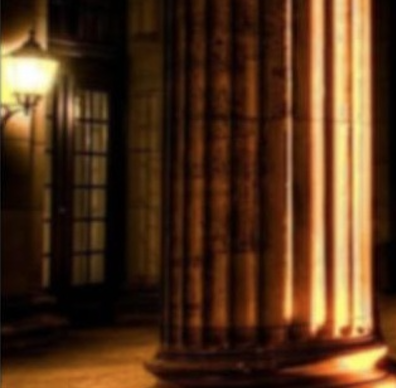
\includegraphics[width=7cm, height=7cm]{a}
	\caption{Blurriness: 0.8086}
	\label{default}
	\end{subfigure}
	%
	\hspace{1cm}
	%
	\begin{subfigure}[b]{0.49 \textwidth}
	\centering
	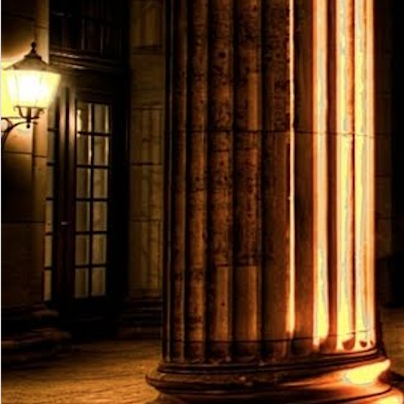
\includegraphics[width=7cm, height=7cm]{b}
	\caption{Blurriness: 0.3648}
	\label{default}
	\end{subfigure}
\caption{Blurriness measure compare}
\end{figure}
\par
The blockiness is measured by using the method of Wang et al. which estimates the average difference across block boundaries modulated by image activities \cite{Wang}.
\begin{figure}[h]
	\begin{subfigure}[h]{0.49 \textwidth}
	\centering
	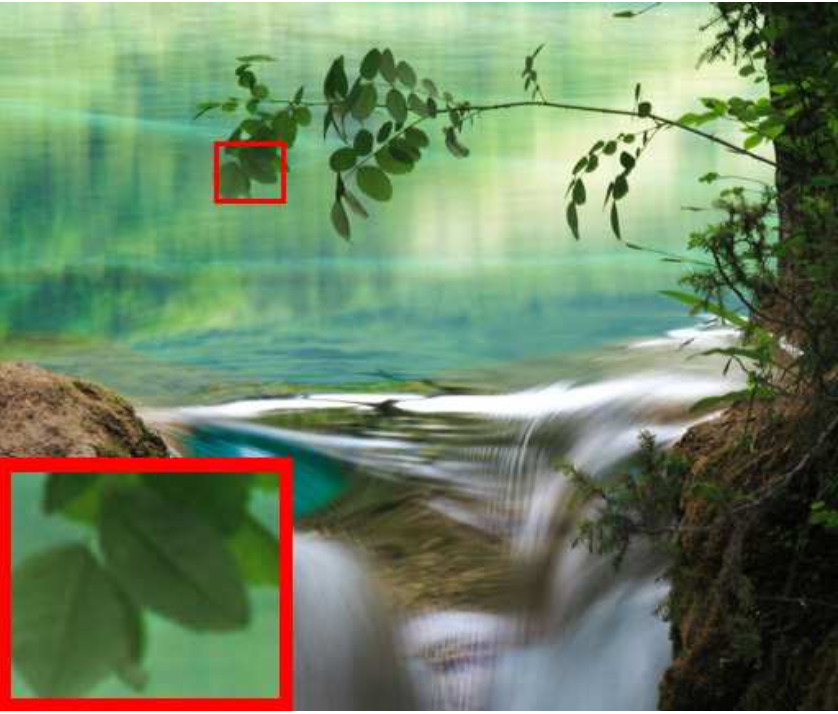
\includegraphics[width=7cm, height=7cm]{a1}
	\caption{Blockiness: 0.204}
	\label{default}
	\end{subfigure}
	%
	\hspace{1cm}
	%
	\begin{subfigure}[h]{0.49 \textwidth}
	\centering
	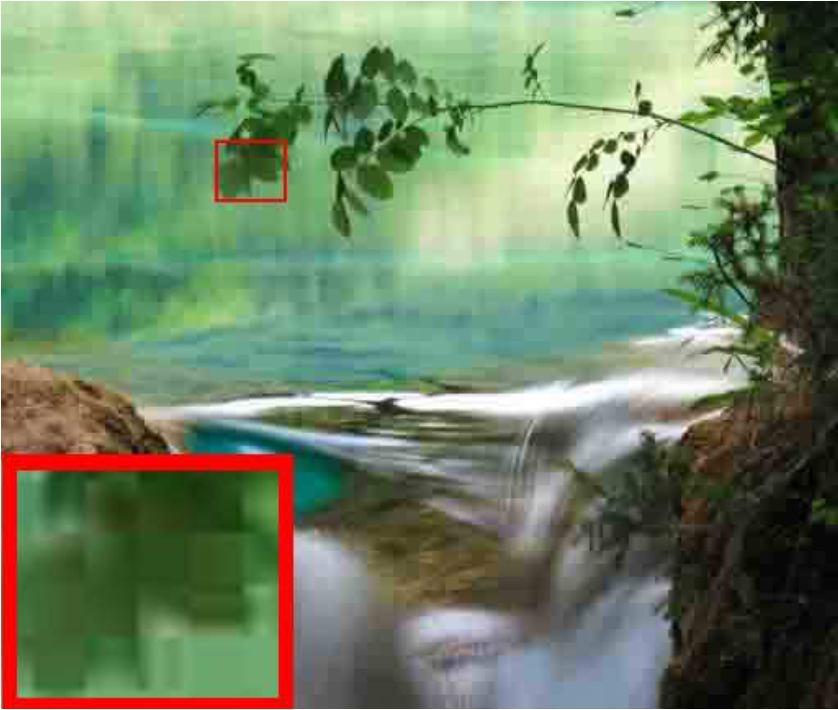
\includegraphics[width=7cm, height=7cm]{b1}
	\caption{Blockiness: 0.479}
	\label{default}
	\end{subfigure}
\caption{Blockiness measure compare}
\end{figure}

After obtain the blockiness and blurriness from all the frames within a given video segment, we calculate the visual distortion for this segment as follows:
\begin{equation}
\mathit{E_{vv}(S_i)} = \sum_{\substack{\mathit{I_k\in S_i}}}\gamma \mathit{q_{bk}(I_k)} + (1 - \gamma)\mathit{q_{br}(I_k)}
\end{equation} 
where $\mathit{q_{bk}(I_k)}$ is the measurement of blockiness of given frame, and $\mathit{q_{br}(I_k)}$ is the measurement of blurriness. Weight $\gamma$ is set to 0.45.

\subsection{Incorrectness of Motion Model}
In order to achieve the "mosaicablity", we use a homography to model the motion between frames. By matching SIFT feature points, we are able to locate significant points between frames and thus obtain the homography. In practice, getting a high quality panorama from video requires the inter-frame motion is closed to its homography and few casual videos can achieve that. Therefore, we measure the error using the real motion vector from SIFT feature points and the predicted value by homography between two successive frames.
\begin{equation}
\mathit{E_{vm}(S_i)} = \sum_{\substack{\mathit{I_k\in S_i}}} \frac{1}{\mathit{n_k}} \sum_{\substack{\mathit{p_{j,k}}\in \mathit{S_i}}} \lVert \mathit{mv(p_{j,k})}, \mathit{mv_h(p_{j,k})} \rVert
\end{equation}
We first for each adjacent frame $\mathit{I_k}$ and $\mathit{I_{k + 1}}$ find its matching SIFT feature pairs, and calculate homography using RANSAC based on these feature pairs. The notation $\mathit{mv(p_{j,k})}$ is the motion vector of $\mathit{j^{th}}$ SIFT feature point of frame $\mathit{I_k}$ and $\mathit{mv_h(p_{j,k})}$ is the predicted motion vector by homography at $\mathit{j^{th}}$ feature point. Then the error of $\mathit{j^{th}}$ feature point is taking the L1 norm of these two terms. Then we average the errors of all feature pair in each frame and obtain the incorrectness of motion model by summing up all the average. 
 
 \section{Extent of Scene}
 	The extent of scene $\varepsilon(\mathit{S_i})$ is defined as the scene covered by the video segment. Although it could be good if we maximizing the covering area to obtain a larger field of view, larger field of view often means more distortion. Hence, we want to choose the reference frame where the distortion is minimum, in other words, we want the minimum area covered by segment $\mathit{S_i}$
	
\begin{figure}[h]
	\centering
	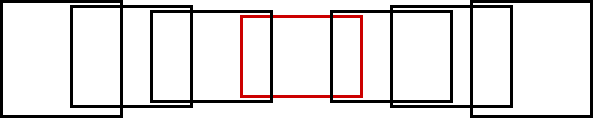
\includegraphics[width=15cm]{reference}
	\caption{All the other frames in the video are alignment to the reference frame, and we want to find the optimal reference frame so that the area covered by aligning all the frames to be minimized}
\end{figure}

In order to find the optimal reference frame, we want to search for all possible combination of panorama alignment as follows:
\begin{equation}
\mathit{r} = \mathrm{arg} \min_{\mathit{f_r} \in \mathit{S_i}} \bigcup_{\mathit{f} \in \mathit{S_i}} \mathit{I(f, f_r)}
\end{equation}
Then the extent of scene is defined as:
\begin{equation}
\varepsilon(\mathit{S_i}) = \bigcup_{\mathit{f} \in \mathit{S_i}} \mathit{I(f, r)}
\end{equation}
In Lui et al. paper, they used generic polygon clipping for finding the minimum area covered. However, we used another approach.  Although the accuracy declines, the complexity reduces in decent amount, we choose to find the distance between the center of reference frame and that of all other frames as follows:
\begin{equation}
\frac{1}{\mathit{n}} \sum_{\mathit{f \in S_i}}  \lVert \mathit{C_r}, \mathit{C_f} \rVert
\end{equation}
Where $\mathit{n}$ is the number of frames within the segment, $\mathit{C_r}$ is the center pixel of the reference frame and $\mathit{f_r}$ is the center pixel in a given frame.
\begin{figure}[h]
	\centering
		\begin{subfigure}{1\textwidth}
		\centering
			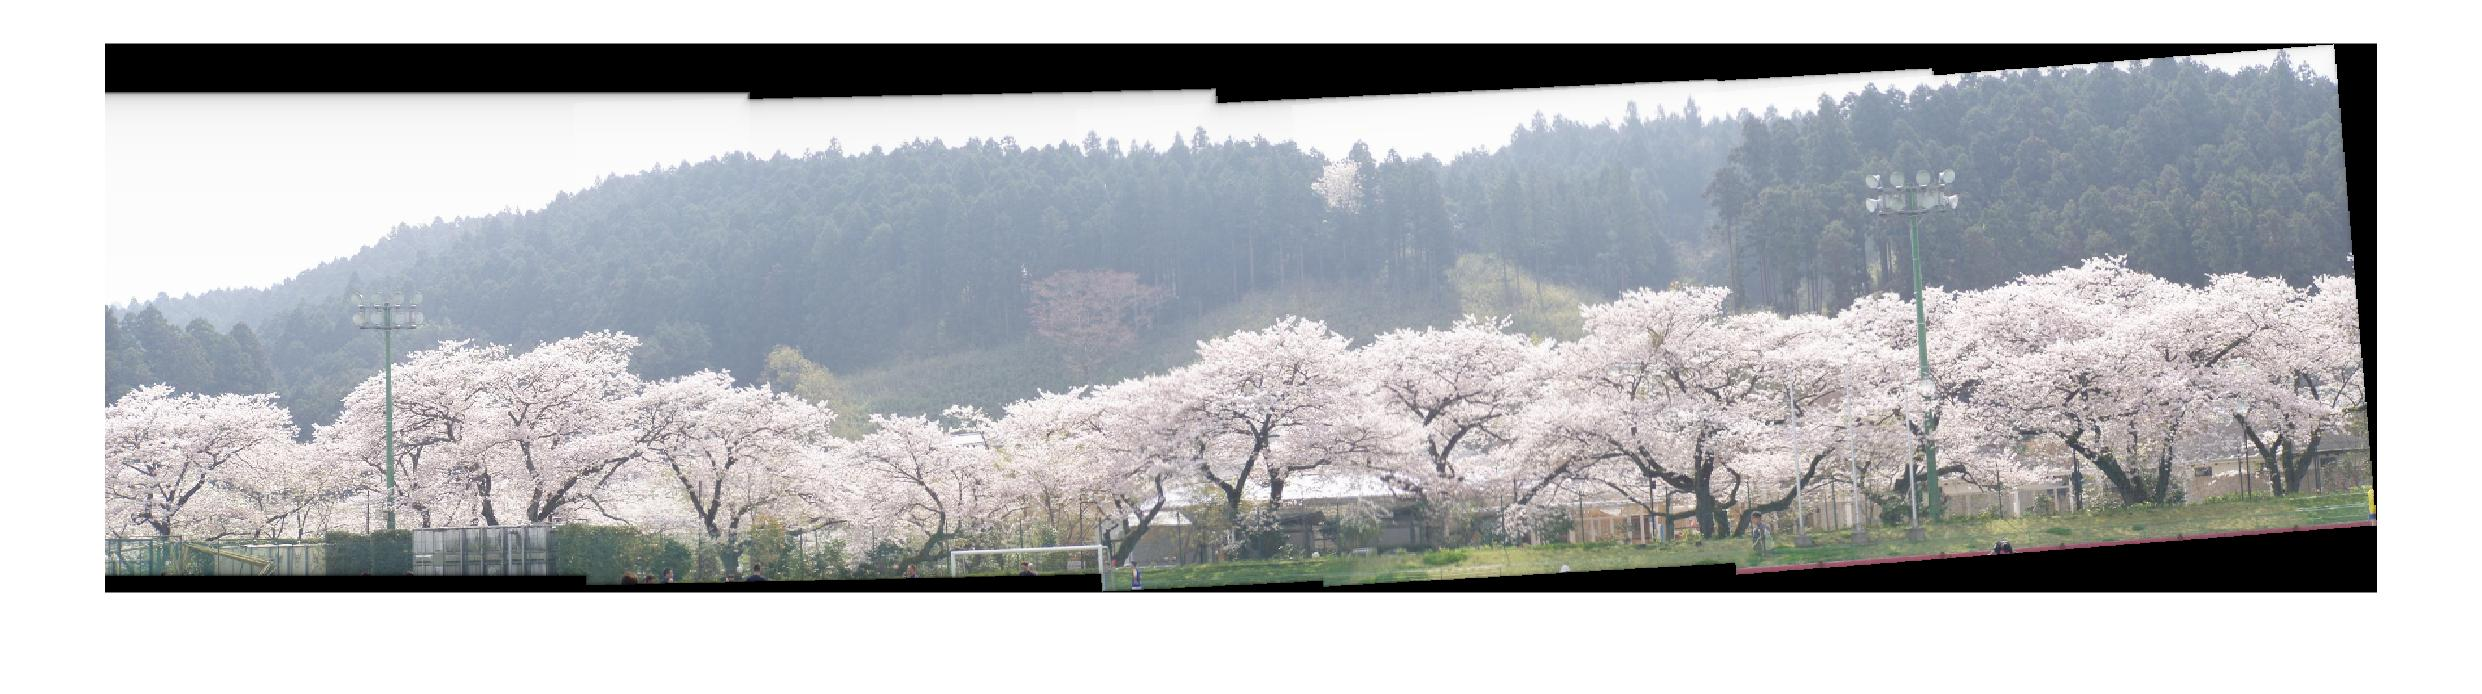
\includegraphics[height=3.5cm, width=15cm]{ref1}
			\caption{The reference frame is set at the left most frame}
			\label{fig:ref1}
		\end{subfigure}
		~
		\begin{subfigure}{1\textwidth}
		\centering
			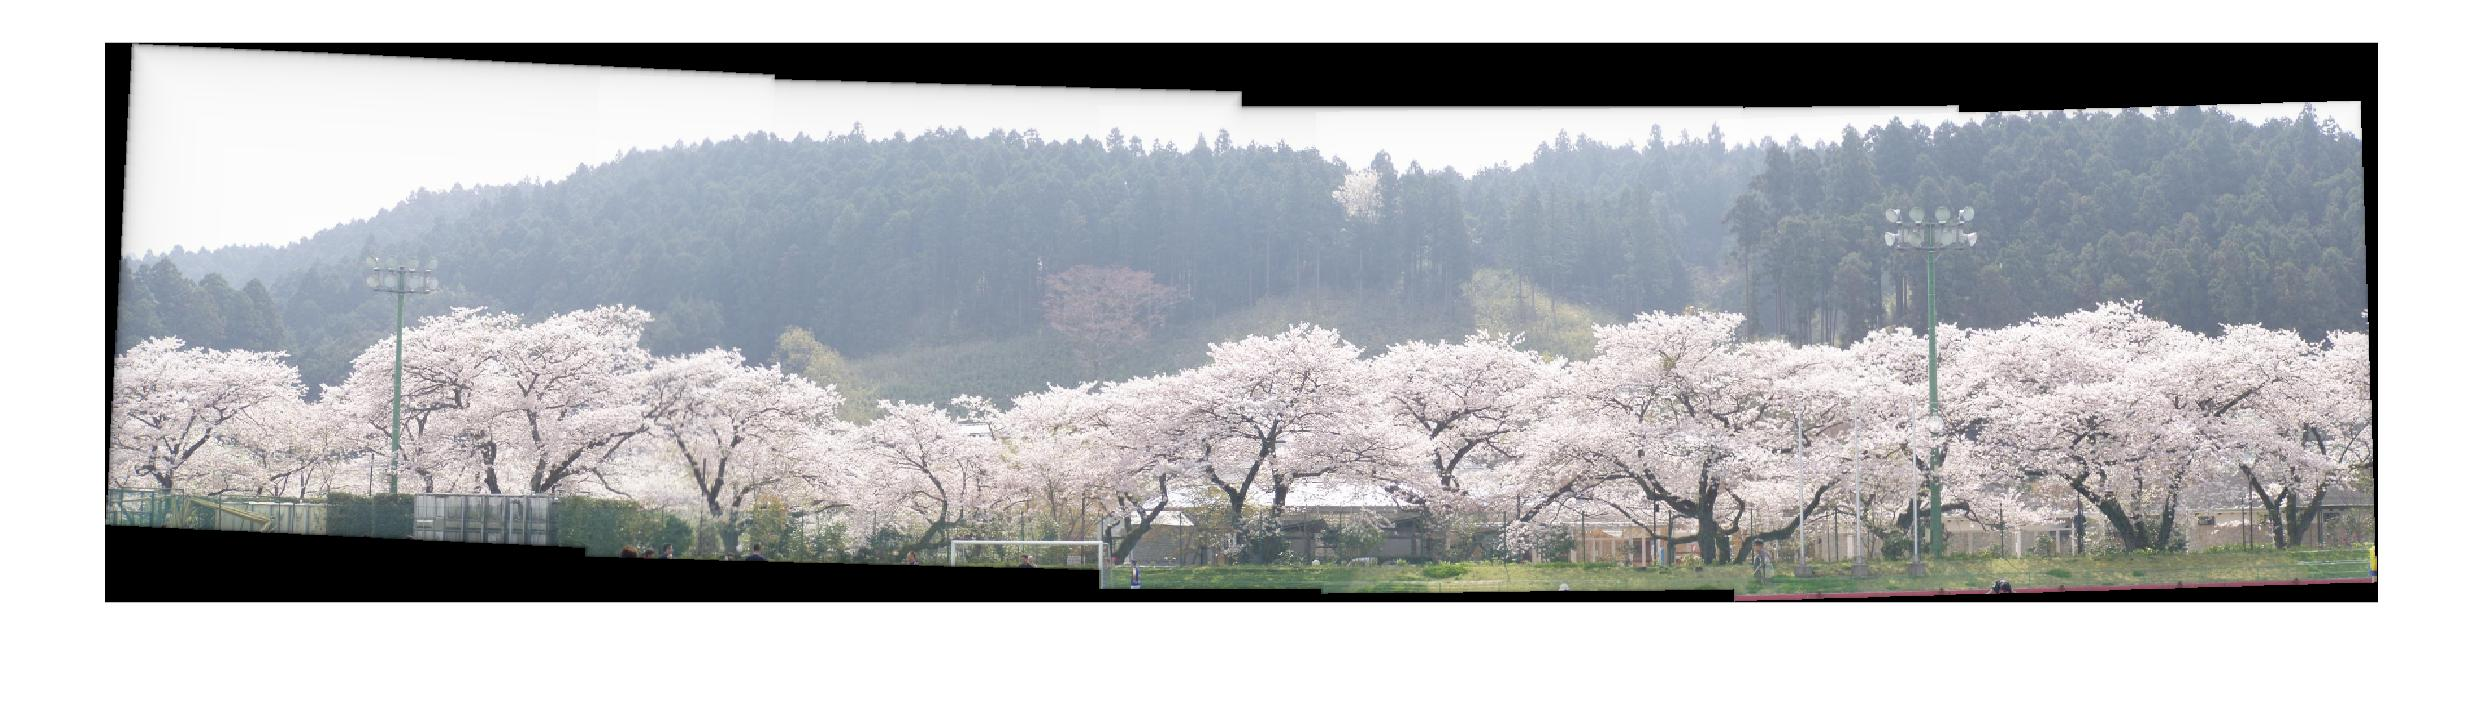
\includegraphics[height=3.5cm, width=15cm]{ref3}
			\caption{The reference frame is set at the center frame}
			\label{fig:ref3}
		\end{subfigure}
		~
				\begin{subfigure}{1\textwidth}
		\centering
			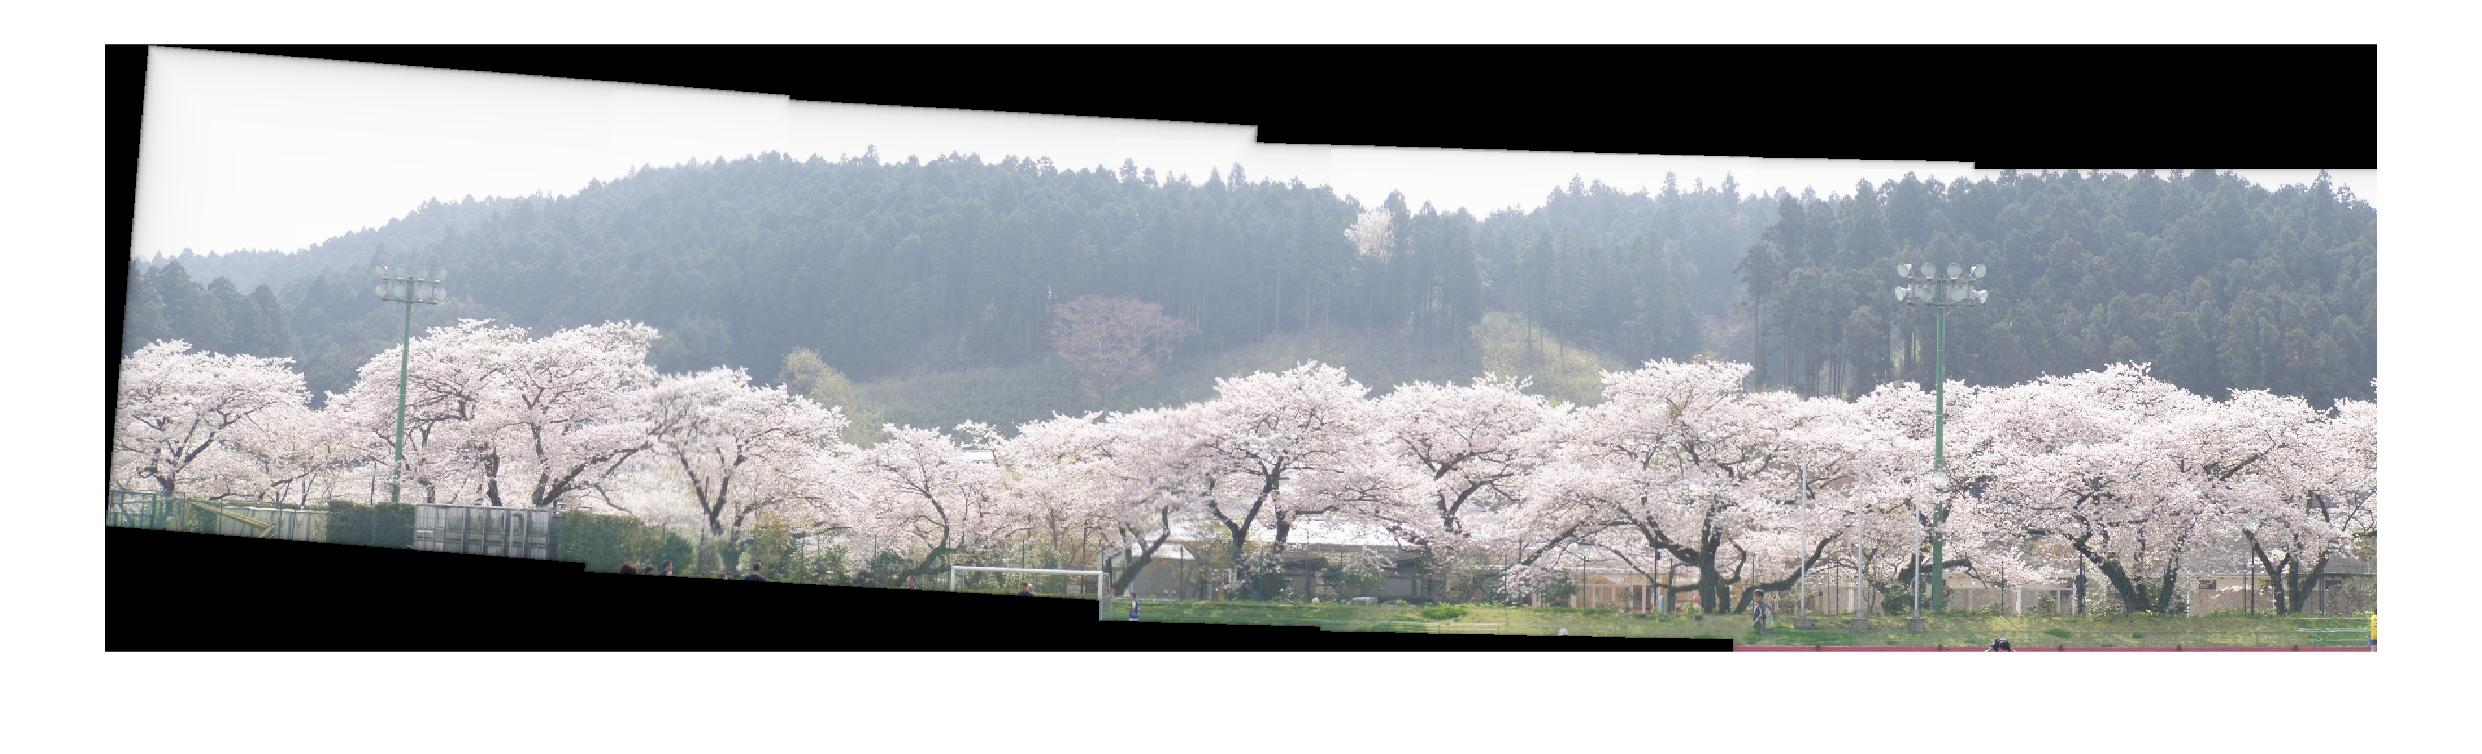
\includegraphics[height=3.5cm, width=15cm]{ref5}
			\caption{The reference frame is set at the right most frame}
			\label{fig:ref5}
		\end{subfigure}
		\caption{Difference reference frame results in different look of panorama}
\end{figure}
Figure 4 demonstrates when reference frame is the most left frame (the first frame in the image sequence), the middle frame and the right most frame. However, due to the relatively small distortion since this image sequence only has 5 images, the visual difference between three panoramas is subtle. 

\section{Experiments and Results for Determining Panorama}
We randomly select some videos from Youtube and manually cut the video into several segments. Lui et al. use histogram based shot boundary detection to divide the video, and we use another approach which we will describe in next section. In order to test the correctness of the three panorama synthesis criteria, we choose to feed our algorithm with preprocessed video segments.\\
\\
\begin{figure}[h]
	\centering
	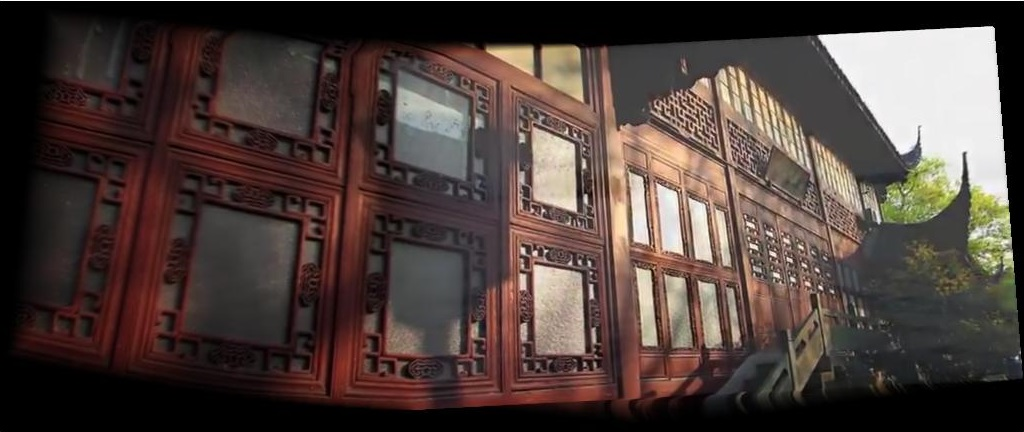
\includegraphics[width=9.5cm, height=3cm]{building562-691}
	\caption{Stitched using a video segment from West Lake}
\end{figure}\\
In figure 5, the motion error we estimated is 598 (rounded to nearest integer) and since this segment has over 130 frames, so on average each frame has 4.6 error which is considered a good score in our standard. The image quality error for this segment is 23 which is also a relatively good score for a 360p video. Therefore, we obtained a decent panorama from this segment.
\begin{figure}[h]
	\centering
	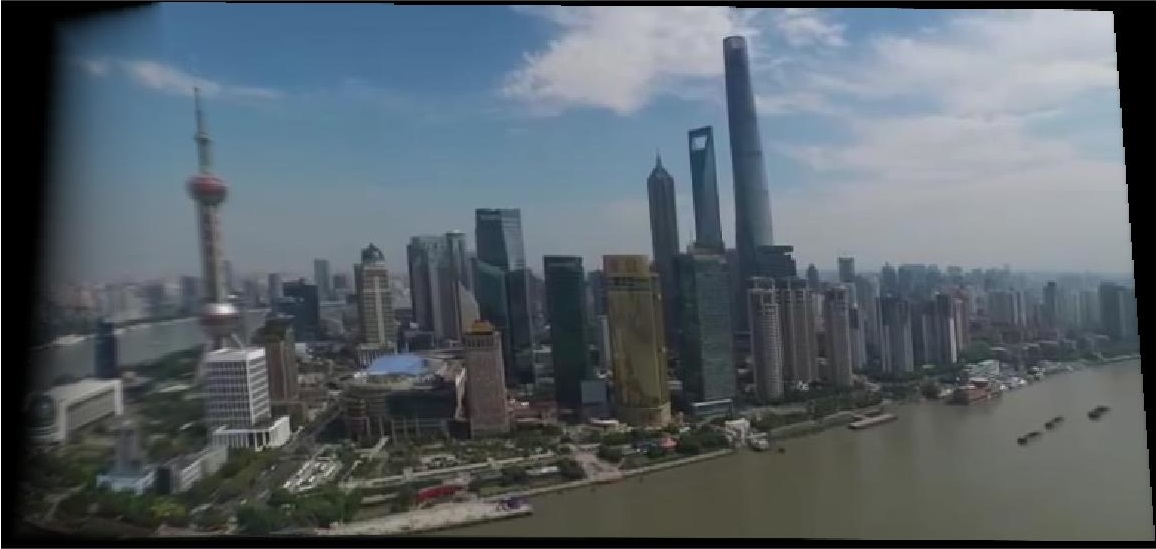
\includegraphics[width=9.5cm, height=3cm]{shanghai1309-1440}
	\caption{Stitched using a video segment from Shanghai shot by drone}
\end{figure}
Figure 6 shows a shot from Shanghai, and the computed motion error is 587. Because the drone is very stable in the original video, the motion error is also what we expected. We also discovered that the image quality error of 360p videos from Youtube usually ranges from 20 to 45. Therefore, the panorama synthesized is also in good quality with only a subtle distortion. 
\begin{figure}[h]
	\centering
	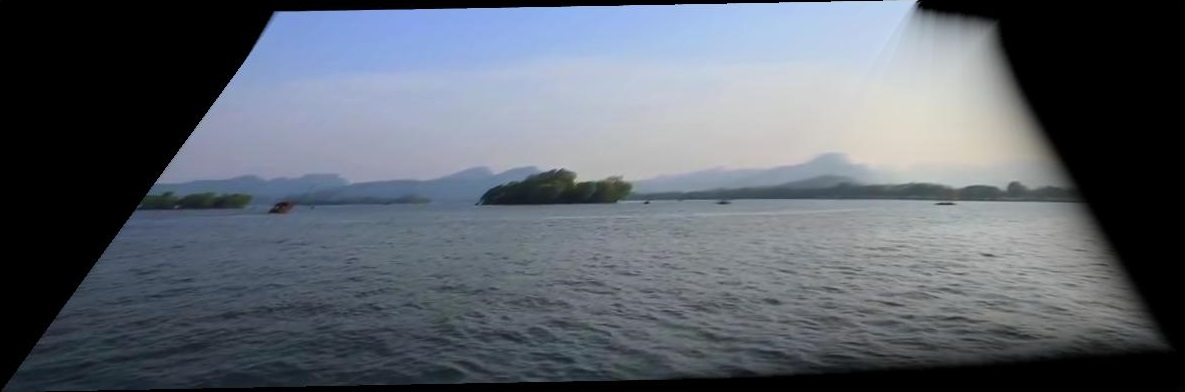
\includegraphics[width=9.5cm, height=3cm]{lakeError1206-1310}
	\caption{Stitched using a video segment from West Lake}
\end{figure}\\
Figure 7 is a failure. In the segment, we observed a large amount of object motion which is from the waves and the boats on the lake. As a result, the motion error for this segment is 1521. In addition, due to the panorama. 
As a conclusion, our implementation of judging a segment works as expected and is able to distinguish between segments with different quality.

\section{Video Segment Fetching}
Lui et al. preprocess the given video by applying histogram based method for shot boundary detection and shot boundary is detected whenever the histogram intersection between two adjacent frames is below a threshold. 
However, we detect scene boundary by using the visual quality distortion.The idea is that in order to calculate the homography between two adjacent frames, we should have at least 4 SIFT matching pairs. According to our experiments, the video segments we have do not always have enough pairs to calculate homography when two frames are at scene boundary and even when they have enough pairs to calculate the visual quality error tend to be high. Thus, we cut the whole video into 20 frames segments, then compute visual quality error for each segments and by setting the visual quality error to infinity when encounter scene transition segment and dropping that segment we are able to append all adjacent segments to obtain a optimal segement for panorama stiching. \\
We define the types of videos that we might encounter while fetching as follows: \\
\\
Case 1: A scene that is not capable of synthesizing panorama (bad scene) followed by a scene that is proper source for panorama (good scene) or a good scene followed by a bad scene, in both cases we want to only obtain one panorama from the good scene:
\begin{figure}[h]
	\centering
	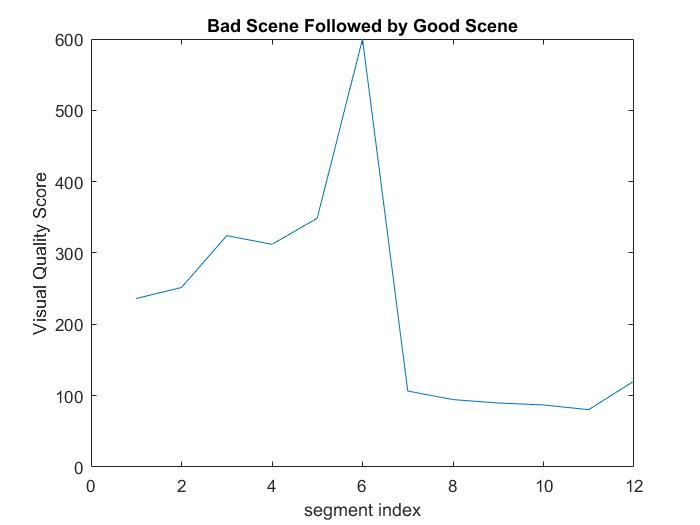
\includegraphics[width=10cm]{bad-good-fig}
	\caption{Visual quality error for Case 1}
\end{figure}\\
Above figure shows that the overrall visual quality error for bad scene segments are high (over 250) and we have this sudden increase in the error at segment 6, thus we can say segment 6 has a high possibility of containing a scene transition. And we want drop all the segments before segment 7 due to high error and synthesize panorama use only segment 7 to 12.\\
Case 2: A good scene followed a good scene followed. In this situation, we want to get two panoramas :
\begin{figure}[h]
	\centering
	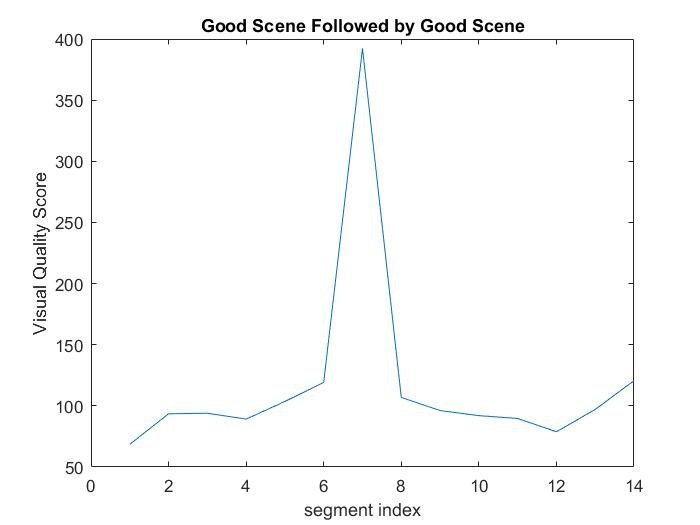
\includegraphics[width=10cm]{good-good-fig}
	\caption{Visual quality error for Case 2}
\end{figure}\\

It can be observed that before and after segment 7 there are two smooth segments series and a sudden increase in visual quality error at segment 7. In this case, we want to drop segment 7 and synthesize two panoramas from segment 1 to 5 and segment 7 to the rest segments.\\
Case 3: A bad scene followed by a bad scene. In this situation, we want to drop both scenes, and we can expect the overrall visual quality errors are relatively high across all the segments.
\section{Limitations}
First of all, the whole process is significantly very time consuming. Because we are computing the visual quality score in each segments due to our segmentation algorithm, the complexity tends to be very large. During our experiments, a 250 frames video will take raghly 40 seconds to process. Another limitation is that because we are dropping the whole 20 frames segment with scene transition the field of view of the final panoramas are reduced in small amount. 
\end{document}
